\chapter{FTS transfer failure analysis} \label{sec:pipeline}

The general idea is to start from a collection of textual data, corpus, formed by documents of various lengths and scope.
The available information is then analyzed to retrieve groups of documents sharing similar content, and the matching patterns are interpreted as topic descriptions.
Of course, the string format of the raw data is highly unstructured and impractical to handle, thus limiting the plethora of applicable techniques. 
For this reason, the (possibly long) strings incorporated in the documents are first quantized into unitary pieces of textual information, tokens, from which the raw strings can be reconstructed. These process may vary from simply using words \cite{bengio2003word, mccann2017word} or characters \cite{ling2015char, dhingra2016char}, to more complex strategies involving subwords \cite{gage1994subword, sennrich2016subword}, sentences \cite{kiros2015sentence}, documents \cite{le2014documents} and topics \cite{niu2015topic}. 



Our work is inspired by the approach described in \cite{lin2016log}, although only part of the pipeline has been developed since no knowledge base is available for our use case.
Also, our work is conceptually similar to the work of \cite{clusterlog2021}, although some major differences are present in the pre-processing, clustering and description stages.

\sidenote[Luca][notesyellow]{Confronto con pipeline di Maria e argomentazione differenze}
Although this pipeline accounts for most needs of typical workflows concerning error messages, it also presents some drawbacks.
First, the pre-processing and vectorization stages reduce all the principal sources of variability, turning the whole approach into something close to unique strings grouping (assuming a smart and flexible definition of unique strings). 
For example,  the raw error messages are transformed into structured templates where the same placeholder replaces parametric parts.
This choice drastically decreases the data variability. Also, it hampers the usage of parameter values for error discrimination, potentially masking faults due to specific components, e.g. one particular file is corrupted and needs restoration, or a determined site/service is not responding.
Moreover, performing principal components decomposition on the word2vec embedding further reduces the expressive power of the learned representation.
Although the previous strategies are crucial to comply with the runtime and computing requirements of particular use cases, they seem to contrast the current best practice for text processing. 
In fact,  the recent applications of Natural Language Processing (NLP) suggest exploiting the increased computing power of modern architectures to train bigger models with minimal hard-coded pre-processing. 
The idea behind that is to let the model figure out linguistic features -- e.g. grammar, syntax, lexicon, semantic -- relations among tokens, thus endowing the resulting model with increased expressive power.
As a result, the previous strategies likely hinder learning an optimal embedding, perhaps questioning the need for the word2vec language model for text vectorization in the first place.
As a second drawback, no auxiliary information concerning the precesses is considered alongside the error message. 

One of the main concerns in data transfer operations is to promptly detect and solve issues that affect the functioning of the infrastructure.
On our way towards improving automation of DDM operations, we adopted an unsupervised learning approach to minimise experts' effort and enable discovering new failure patterns related to FTS transfers. 
The pipeline consists of 
% can be summarised into 
two main steps: \textit{i)} vectorization and \textit{ii)} clustering.
In the {\emph{vectorization step}} we concatenate the raw error string with source and destination hostnames and we use a word2vec model that learns how to map all that information to a vectorial space of a given size, where similar errors are expected to be close together. This is to transform the textual information into a convenient numeric representation and serves as preprocessing for the next steps. 
A {\emph{clustering algorithm}} is then applied to group related errors: 
% In practice, the idea is to 
we pre-train a word2vec model on a big dataset 
-- possibly updating it once in a while -- and then 
and run a \mbox{K-Means++} algorithm \cite{kmeans} online during the monitoring shifts.  
% 

In order to demonstrate the approach, we report an analysis of FTS data from one full day of operation. %(15/01/2021).
\cref{fig:cluster0} shows an example of a summary table for the biggest cluster found by the model.
\begin{figure}[t]
    \centering
    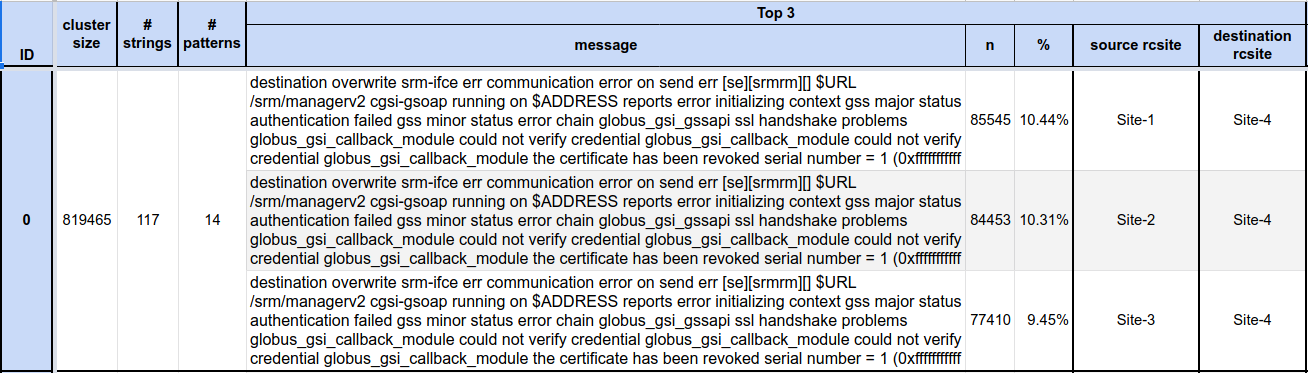
\includegraphics[width=\textwidth]{figures/410_method/cluster0_wide.png}
    \caption{
    % Example of cluster summary for cluster 0, the biggest cluster found by the chosen model. % 
    Example of an error message cluster summary.}
    \label{fig:cluster0}
\end{figure}
The first three columns provide numeric summaries: \textit{i)} the cluster size, \textit{ii)} the number of unique strings within the cluster, and \textit{iii)} the number of unique patterns: unique strings after the removal of parametric parts like paths, IP addresses, URLs and so on. The model learns to \textit{abstract} message parameters and to group strings that are similar except for the parametric parts. As a result, the initial amount of errors is reduced to a number of patterns which is lower by several orders of magnitude. 
The core part of this visualization is then represented by the \textit{Top 3} section, where the most frequent triplets of pattern, source and destination sites are reported in descending order, together with their multiplicity and the percentage over the cluster size.
There we extract several insights, for example whether a pattern is responsible for a large number of failures or if it accounts for a conspicuous fraction of the cluster. In addition, one can investigate the contribution of source/destination site pairs, 
% Also, one could look at whether errors are concentrated in a specific source/destination site, 
as in \cref{fig:cluster0} where Site-4 clearly seems to have a problem as destination. 
%
Another useful piece of information is given by the cluster's time evolution plot (shown in \cref{fig:timeplot_cluster0}) that can give an immediate indication of whether the problem  is transient or not. 

% \begin{wrapfigure}{hR}{0.53\textwidth}
\begin{figure}
    \centering
    % \vspace{-8mm}
    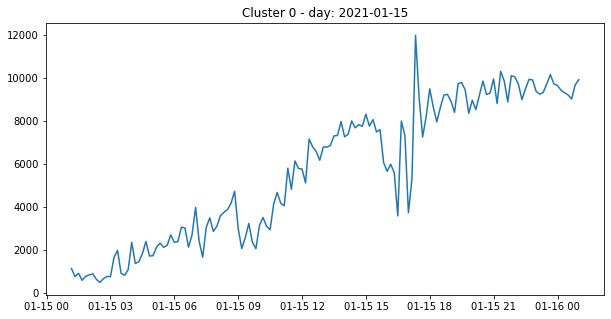
\includegraphics[width=\textwidth]{figures/410_method/timeplot_cluster0.png}
    \caption{Time evolution of cluster 0: the plot shows the count of errors in bins of 10 minutes.\vspace{3mm}\phantom{.}}
    \label{fig:timeplot_cluster0}
    % \vspace{-10mm}
\end{figure}
% \end{wrapfigure}

%
Overall, the idea is for the shifters to look at summary tables and time plots for each of the clusters detected by the algorithm, which act as suggestions of possible issues to investigate further, or later, would create automatic alerts, notifications, or even issue reports. 

\newcommand{\specialcell}[2][c]{\begin{tabular}[#1]{@{}c@{}}#2\end{tabular}}
\begin{table}[htb]
\centering
% \resizebox{\textwidth}{!}{
\begin{tabular}{cccccccc}
\toprule
\textbf{N. Clusters} &  \textbf{ASW} &  \textbf{WSSE} &  \textbf{\specialcell{Perfect\\Match}} &  \textbf{\specialcell{Fuzzy\\Match}} &  \textbf{\specialcell{Partial\\Match}} & \textbf{\specialcell{False \\ Positives}} & \textbf{\specialcell{False \\Negatives}} \\
\toprule
     &       &        &     &    &    &    &   \\[-0.25cm]
  15 &  0.89 &  17107 &   7 &  3 &  2 &  3 &  1 \\[0.2cm]
\bottomrule  
\end{tabular}
% }
\caption{Summary of pre-validation results.}
\label{tab:crosscheck}
\end{table}

The process described above can be fully automated after tuning model hyper parameters based on metrics such as Average Silhouette Width score
% (ASW)
and Within-cluster Sum of Squared (Euclidean) distances, that measure how compact and separated the clusters are.
However, this is not directly related to the meaning of the messages being grouped. Hence, this is to be intended as a proxy of a correct model behaviour rather than a real performance metric.
For this reason, 
We have conducted an extensive testing as pre-validation comparing the clusters obtained with this approach against GGUS tickets, showing a reasonable overlap between suggested and reported issues. 
In particular, for the analysis above we considered issues reported in a skewed time window of 17 days (1st to 18th January) so to include both known issues and the ones possibly spotted with some delay.
Results of this cross-check are reported in Table \ref{tab:crosscheck}.

The model found 15 clusters reaching ASW and WSSE of 0.89 and 17107, respectively. The results show a good agreement, with 7 perfect matches (both reported message and affected site), 3 fuzzy matches (i.e., the cluster had evident connection with more than one ticket) and 2 partial ones (either message or site). Besides that, 3 clusters highlighted issues that were not reported on GGUS. In some cases, posterior checks showed hints for real problems that went undetected or unreported by experts. %%Finally, 1 GGUS ticket was not discovered by the algorithm. 
% 
Although it makes sense to cross-check clustering results with tickets, this comparison has some drawbacks. In particular, the procedure is very sensitive to the choice of the time window.
% (some issues could have no match because already reported days before or because yet to be detected on the day of the analysis)
It requires a manual check of the ticket information and the cluster content, which makes the comparison lengthy and not scalable.
% For this reason, we are planning
% 
% Therefore we intend to build a reference dataset where to store labels for error categories, root causes, priority and solving actions. In this way, we will have a real measure of performance while easing the comparison of alternative algorithms and making the investigation of novel techniques sustainable.
% More importantly, collecting such information would allow leveraging tools available in NLP literature about Question Answering (QA) or Named Entity Recognition (NER) to address the key problem related to transfer failures, i.e., understanding the root causes and suggesting solving actions for the problems.

